\documentclass[12pt]{article}

\usepackage{graphicx}% Include figure files
\usepackage{dcolumn}% Align table columns on decimal point

% Use Arial font %
\usepackage{helvet}
\renewcommand{\familydefault}{\sfdefault} 

% Default margins and paper properties %
\usepackage[a4, portrait, margin=0.6in]{geometry}

\begin{document}
	\title{Hypothesis plots summary} % Force line breaks with \\
	\author{1666957, Gustavo Espinal Lugo}
	\date{\today} % It is always \today, today, %  but any date may be explicitly specified

	\maketitle
	%\tableofcontents
	
	\section*{Plots and corresponding metadata}
	mean expected W mass: 80.379 $[GeV/c^{2}]$,\\
mean hypothesis masses: [78.  78.5 79.  79.5 80.  80.5 81.  81.5 82. ] $[GeV/c^{2}]$,\\
mass width: 2.07 $[GeV/c^{2}]$,\\
chi\_square value of hypothesis fit: 11.928241497862004\\
	Absolute path to figure: /home/physics/phuxdp/Desktop/PX402 Physics Project/WBosonProject/T2W5/plots/muPT\_80.379\_2.07\_between\_78\_and\_82\_summary.png\\
	Next lines are the data of the shown histograms (if needed): \\
	All quantities: 	80.379, [78.  78.5 79.  79.5 80.  80.5 81.  81.5 82. ], 2070, 11.928241497862004\\
	X\_energ\_vls = [0.6, 1.7999999999999998, 3.0, 4.199999999999999, 5.4, 6.6, 7.8, 9.0, 10.2, 11.399999999999999, 12.6, 13.799999999999999, 15.0, 16.2, 17.4, 18.6, 19.799999999999997, 21.0, 22.2, 23.4, 24.6, 25.799999999999997, 27.0, 28.199999999999996, 29.4, 30.6, 31.799999999999997, 33.0, 34.2, 35.4, 36.599999999999994, 37.8, 39.0, 40.2, 41.4, 42.599999999999994, 43.8, 45.0, 46.2, 47.4, 48.599999999999994, 49.8, 51.0, 52.2, 53.4, 54.599999999999994, 55.8, 57.0, 58.199999999999996, 59.4, 60.599999999999994, 61.8, 63.0, 64.19999999999999, 65.4, 66.6, 67.8, 69.0, 70.19999999999999, 71.4, 72.6, 73.8, 75.0, 76.19999999999999, 77.4, 78.6, 79.8, 81.0, 82.19999999999999, 83.4, 84.6, 85.8, 87.0, 88.19999999999999, 89.4, 90.6, 91.8, 93.0, 94.19999999999999, 95.4, 96.6, 97.8, 99.0, 100.19999999999999, 101.4, 102.6, 103.8, 105.0, 106.19999999999999, 107.4, 108.6, 109.8, 111.0, 112.19999999999999, 113.4, 114.6, 115.79999999999998, 117.0, 118.19999999999999, 119.4]\\
	Y\_data\_bin\_cnts = [0.0, 0.0, 0.0, 0.0, 0.0, 0.0, 0.0, 0.0, 0.0, 0.0, 0.0, 0.0, 0.0, 0.0, 0.0, 0.0, 1.0, 4.0, 380.0, 18697.0, 24357.0, 26241.0, 28211.0, 30345.0, 32615.0, 34482.0, 36546.0, 38193.0, 40391.0, 41249.0, 42924.0, 43306.0, 40312.0, 34673.0, 27104.0, 20329.0, 15304.0, 12006.0, 9561.0, 7798.0, 6346.0, 5180.0, 4474.0, 3765.0, 3178.0, 2706.0, 2314.0, 2052.0, 1798.0, 1611.0, 1392.0, 1257.0, 1076.0, 933.0, 893.0, 751.0, 697.0, 617.0, 531.0, 469.0, 465.0, 425.0, 382.0, 329.0, 315.0, 286.0, 265.0, 237.0, 205.0, 181.0, 212.0, 156.0, 149.0, 159.0, 132.0, 117.0, 122.0, 109.0, 94.0, 76.0, 91.0, 91.0, 86.0, 58.0, 62.0, 66.0, 51.0, 46.0, 49.0, 47.0, 35.0, 42.0, 34.0, 35.0, 27.0, 32.0, 31.0, 30.0, 33.0, 16.0]\\
	Y\_model\_bin\_cnts = [0.0, 0.0, 0.0, 0.0, 0.0, 0.0, 0.0, 0.0, 0.9608225226402283, 1.921647071838379, 0.0, 0.0, 0.0, 0.0, 0.0, 1.921643853187561, 0.0, 8.6474027633667, 353.5817565917969, 18036.53515625, 23481.20703125, 25453.05078125, 27156.79296875, 29054.64453125, 31186.001953125, 33097.3046875, 35098.94140625, 36696.98046875, 38588.1015625, 40181.33984375, 41238.37109375, 41227.80078125, 38789.8984375, 32887.8203125, 25893.154296875, 19499.078125, 14934.619140625, 11685.6875, 9169.94921875, 7425.84326171875, 6262.142578125, 5134.96337890625, 4322.97119140625, 3562.878662109375, 2934.434814453125, 2639.42919921875, 2310.79248046875, 1953.3389892578125, 1676.624267578125, 1502.7166748046875, 1272.1207275390625, 1207.7464599609375, 1035.760498046875, 951.208740234375, 788.8307495117188, 702.3573608398438, 649.5125732421875, 635.100341796875, 577.4513549804688, 476.56585693359375, 419.87762451171875, 379.5233154296875, 337.2475891113281, 303.6190185546875, 307.46234130859375, 241.16592407226562, 229.63621520996094, 240.2052001953125, 222.9103546142578, 218.10617065429688, 176.79115295410156, 159.496337890625, 135.47592163085938, 119.14201354980469, 128.7501220703125, 124.90692138671875, 104.72966766357422, 101.84716796875, 98.96472930908203, 94.16057586669922, 75.90497589111328, 84.5523452758789, 68.21839904785156, 84.55237579345703, 61.492637634277344, 55.72767639160156, 55.72770690917969, 43.23698425292969, 53.8060302734375, 41.31535720825195, 43.23701477050781, 29.78548812866211, 37.47207260131836, 33.628780364990234, 24.02056121826172, 30.74631690979004, 29.785505294799805, 30.746320724487305, 24.020566940307617, 23.05972671508789]\\

    Found optimal massses ($\chi^2$ roots): [80.42768906] $[GeV/c^{2}]$
    Uncertainty [GeV/c^2]: 1.4210854715202004e-14

	\begin{figure}[tb]
		\centering
		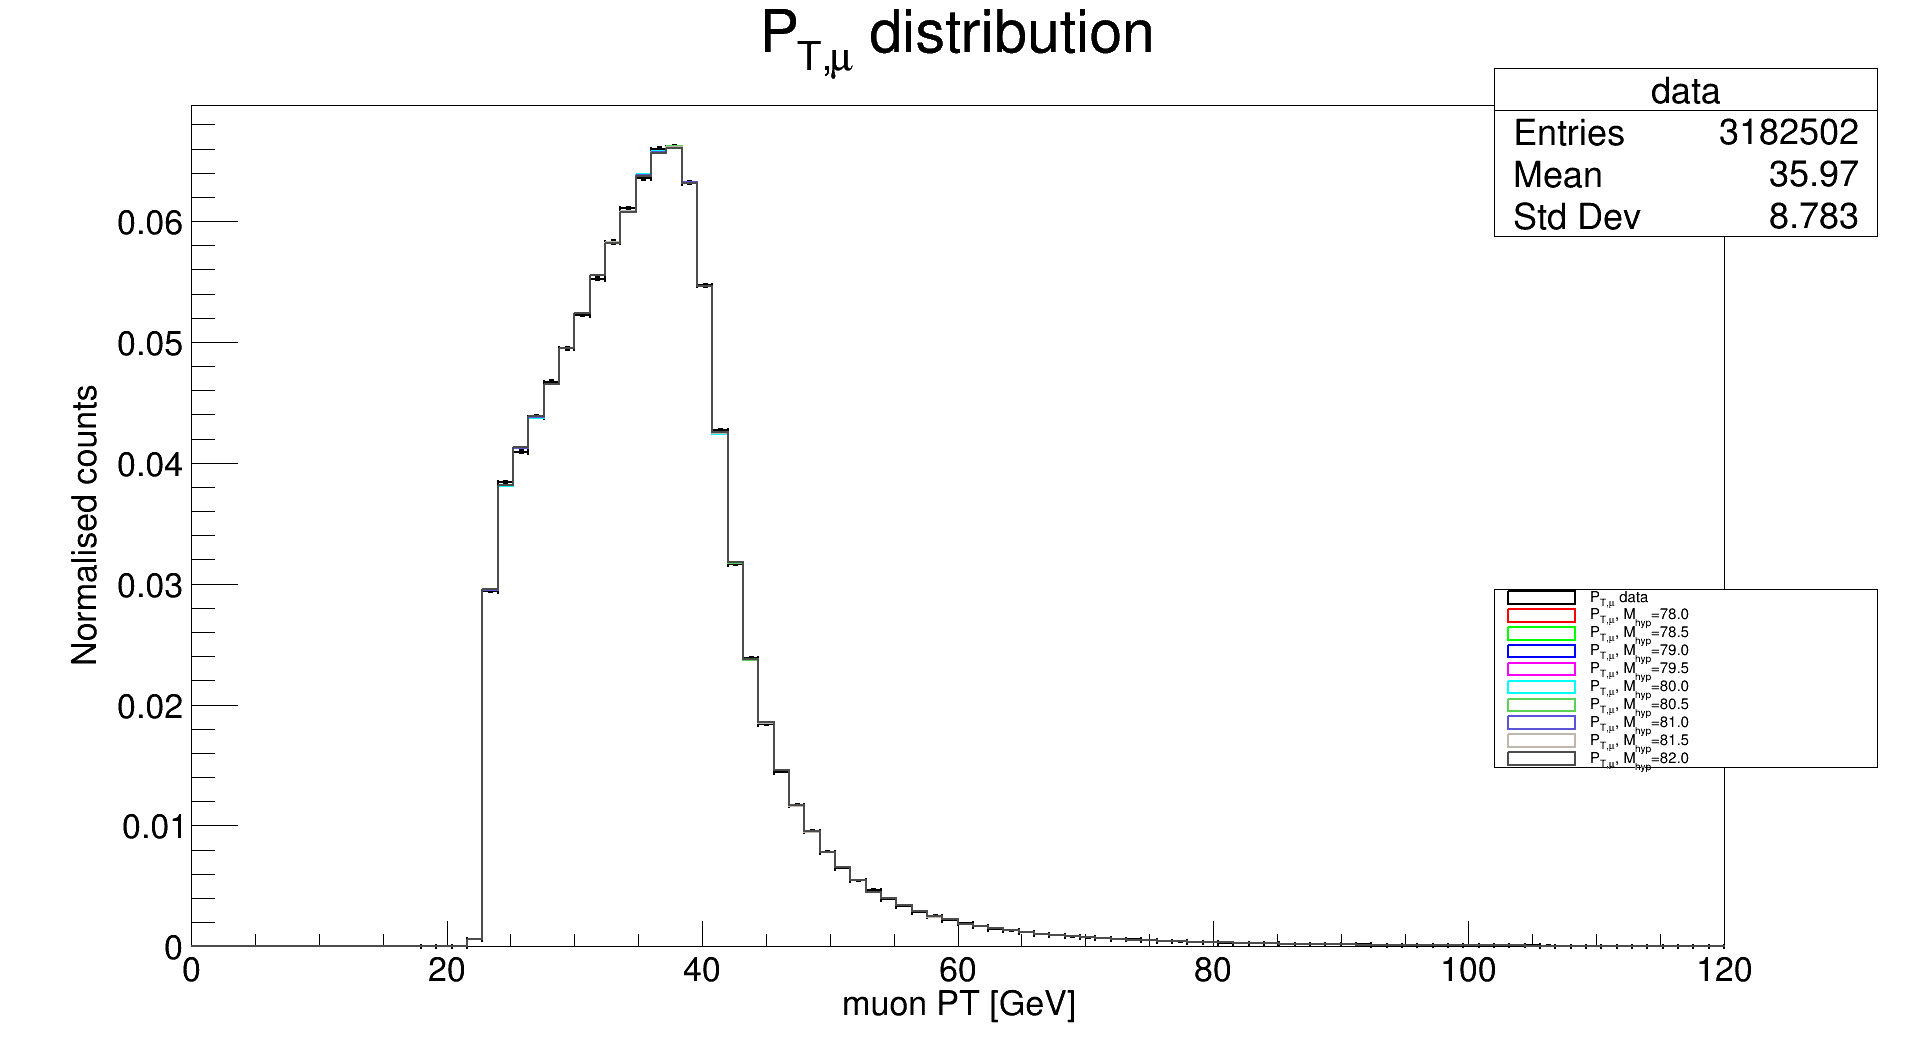
\includegraphics[width=\columnwidth]{/home/physics/phuxdp/Desktop/PX402 Physics Project/WBosonProject/T2W5/plots/muPT_80.379_2.07_between_78_and_82_summary.png}
		\caption{\small Hypothesis masses mean expected W mass: 80.379 $[GeV/c^{2}]$,\\
mean hypothesis masses: [78.  78.5 79.  79.5 80.  80.5 81.  81.5 82. ] $[GeV/c^{2}]$,\\
mass width: 2.07 $[GeV/c^{2}]$,\\
chi_square value of hypothesis fit: 11.928241497862004. }
		\label{fig: fig_0}
	\end{figure}

       \begin{figure}[tb]
		\centering
		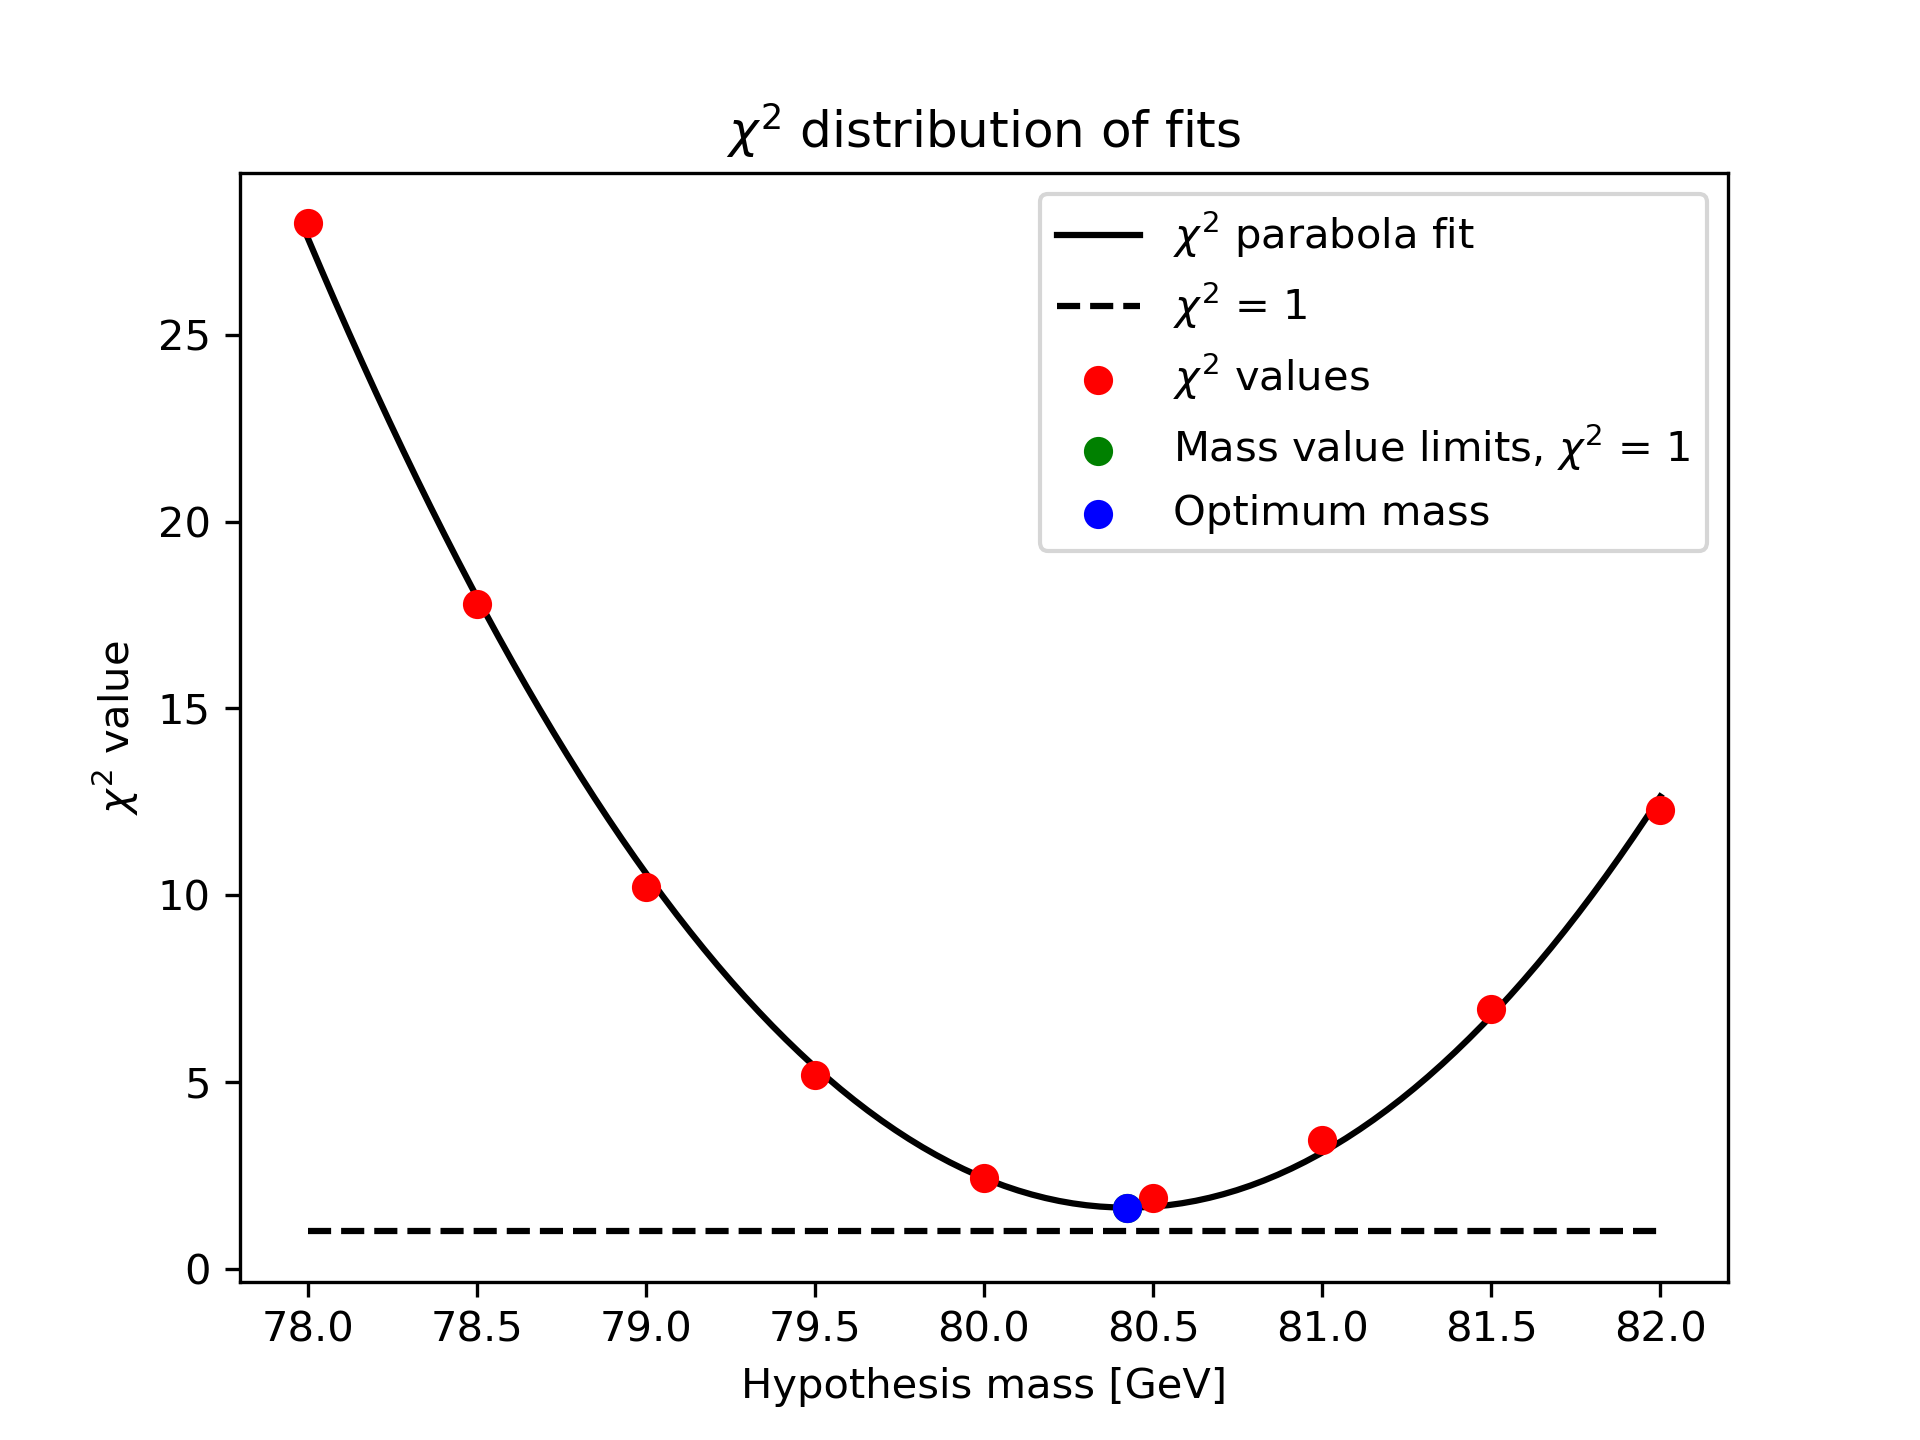
\includegraphics[width=\columnwidth]{/home/physics/phuxdp/Desktop/PX402 Physics Project/WBosonProject/T2W5/plots/chi_square_fits_muPT_80.379_2.07_between_78_and_82_summary.png}
		\caption{\small $\chi^2$ of hypothesis masses. }
		\label{fig: fig_chi_square}
	\end{figure}

    \begin{figure}[tb]
		\centering
		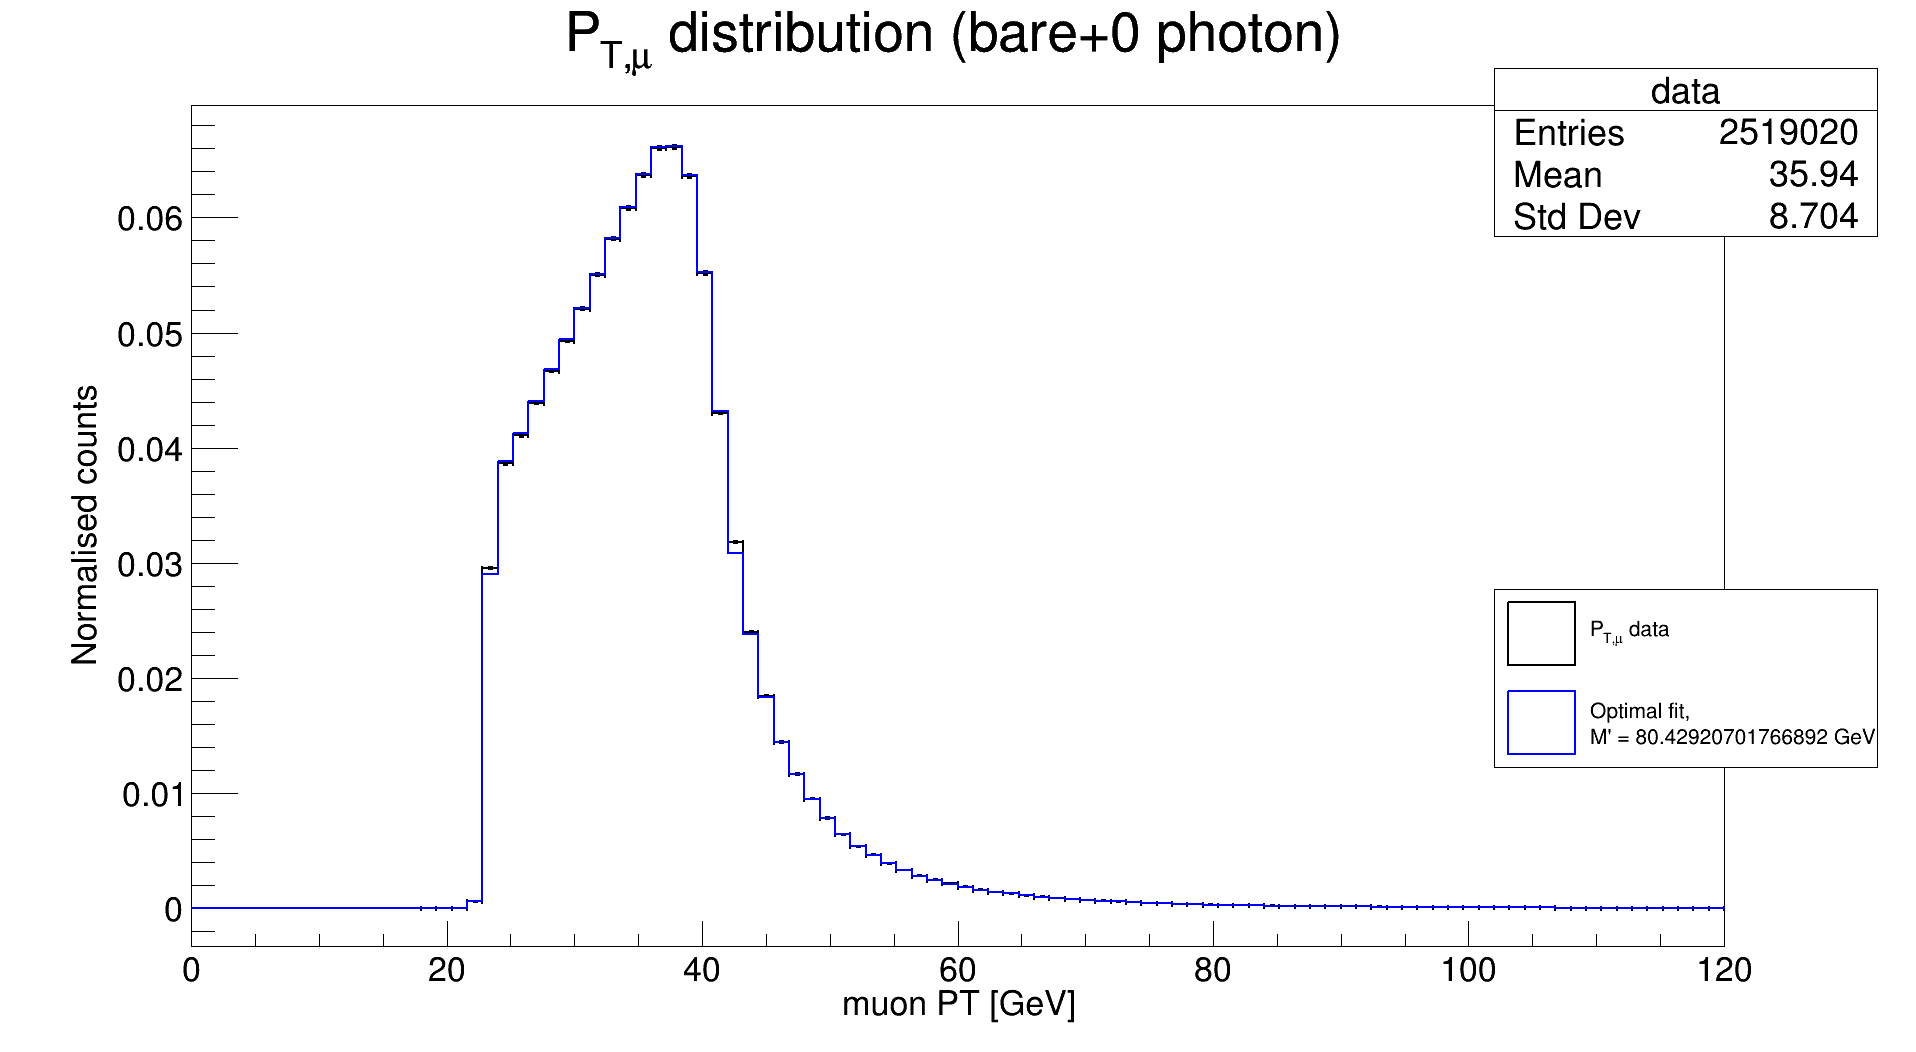
\includegraphics[width=\columnwidth]{/home/physics/phuxdp/Desktop/PX402 Physics Project/WBosonProject/T2W5/plots/optimum_muPT_80.379_2.07_between_78_and_82_summary.png}
		\caption{\small Data and optimum fit with $\chi^2 = 0.02928771495749773$. Used the hypothesis mass of 80.42768906163835$\pm$1.4210854715202004e-14 $[GeV/c^{2}]$. }
		\label{fig: fig_optim_parms}
	\end{figure}
    
\end{document}